% Provenance (never printed): old terminale S material on absolute dating (the
% decay law recalled, the closed system, the rubidium-strontium isochron) and on
% the history of the age of the Earth (cooling, salt, sediments, then radioactivity,
% meteorites and 4.55 billion years). Owner (Sync 0/1): closed system, isochron,
% age of the Earth (as a defined notion). The decay law, the half-life and the
% dating equation are the physics books' (recalled); relative dating, absolute
% age, superposition, cross-cutting relationships and the eras are Book 1 g7's
% (recalled); the oldest zircons and the Acasta gneiss are g12.01's (quoted).
% Varden Hills granite 310 Ma and schist 480 Ma from figdata/shared/region.py;
% their isotope ratios are exercise data (figdata/grade-12/isochrons.py).
\chapter{La datation radiométrique et l'âge de la Terre}\label{ch:g12:age-of-the-earth}

En 1862, le physicien William Thomson, plus tard lord Kelvin, calcula l'\omterm{def:g12:age-of-the-earth:age}{âge
de la Terre} d'après la façon dont elle se refroidit. Il supposa qu'elle
s'était formée en fusion et qu'elle perdait sa chaleur depuis, et chercha
combien de temps il faudrait pour que le gradient de température près de
la surface tombe à sa valeur actuelle. Sa réponse fut 96 millions d'années,
quelque part entre 20 et 400 millions~; en 1897, il ne
retenait plus qu'entre 20 et 40 millions. Les géologues trouvèrent cette durée bien
trop courte pour l'histoire qu'ils lisaient dans les roches. La réponse
vint de la radioactivité, que Kelvin ne connaissait pas.
% ledger: holmes13:estimates, england:kelvin (Book 3 row)

\begin{omfigure}
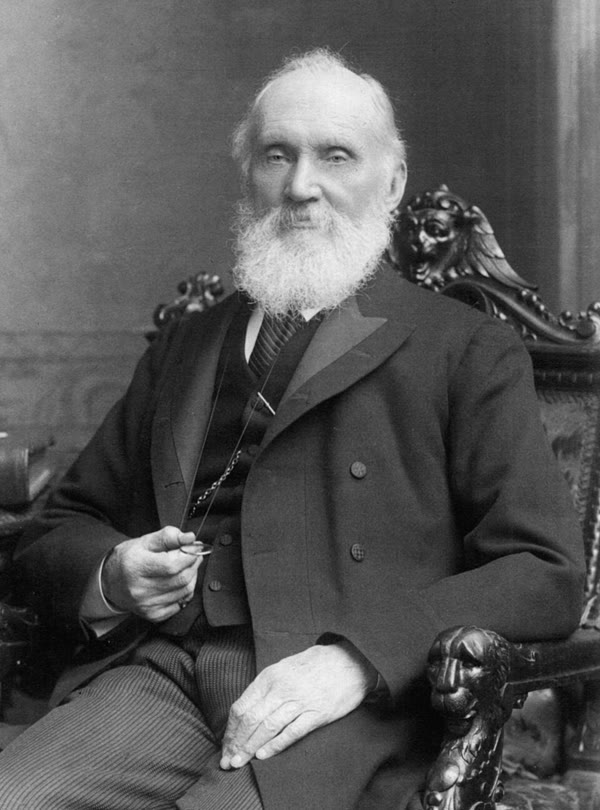
\includegraphics[height=5.2cm]{images/book2/g12-kelvin-1906.jpg}

{\small William Thomson, lord Kelvin, en 1906. Photographie Russell and
Sons, Londres (Smithsonian Institution Libraries, sans restriction de droits
connue).}
\end{omfigure}
% ledger: photo:g12-kelvin

\begin{recall}
La datation relative range les roches et les événements dans l'ordre~; un
âge absolu est un nombre d'années (livre~1, année~7). Un isotope
radioactif, le père, se désintègre au hasard en un isotope fils~: le nombre
$N$ d'atomes pères restants diminue selon
$N = N_0\,e^{-\lambda t}$, où $\lambda$ est la constante de désintégration,
et il est divisé par deux à chaque demi-vie $T = \ln 2/\lambda$ (les livres
de physique). Les plus vieux minéraux connus, des zircons d'Australie-Occidentale,
ont 4.4~milliards d'années (\cref{ch:g12:continental-crust}). La Terre perd
aussi une chaleur que la radioactivité continue de produire, et son manteau
est animé de convection (\cref{ch:g12:internal-heat}).
\end{recall}
% ledger: wilde01:zircon

\section{Une histoire des estimations}

Avant la radioactivité, toute estimation de l'\omterm{def:g12:age-of-the-earth:age}{âge de la Terre} reposait sur
un processus dont on supposait la vitesse connue.

\begin{center}
\small
\begin{tabular}{|p{0.19\linewidth}|p{0.42\linewidth}|p{0.25\linewidth}|}
\hline
qui, quand & méthode et ce qu'elle suppose & estimation \\
\hline
Phillips, 1860 & épaisseur des couches sédimentaires divisée par une vitesse de dépôt~; suppose une vitesse constante & 38 à 96 millions d'années \\
Kelvin, 1862 & refroidissement d'une Terre en fusion par conduction seule, sans source de chaleur interne & 20 à 400 millions d'années \\
G.\,H.~Darwin & temps écoulé depuis la séparation de la Lune et de la Terre, d'après le ralentissement de leurs mouvements par les marées & au moins 56 millions d'années \\
Joly, 1899 & sel apporté à la mer par les fleuves, divisé par l'apport annuel~; suppose un apport constant et aucun sel retiré & 80 à 100 millions d'années \\
\hline
\end{tabular}
\end{center}
% ledger: holmes13:estimates

\begin{history}[La chaleur qui manquait à Kelvin]
En 1903, Pierre Curie et Albert Laborde montrèrent que le radium dégage de
la chaleur, et plusieurs savants soutinrent bientôt que cette chaleur
renversait la conclusion de Kelvin. Un an plus tard, Ernest Rutherford, au
cours d'une conférence à laquelle Kelvin assistait, lui rappela qu'il avait
limité l'\omterm{def:g12:age-of-the-earth:age}{âge de la Terre} «~à condition qu'on ne découvre aucune nouvelle
source de chaleur~». La radioactivité semblait être cette source. Ce
n'était pourtant pas la principale erreur de Kelvin~: ce qui allonge le
plus le refroidissement de la Terre, c'est la \omterm{def:g12:internal-heat:convection}{convection mantellique}, qui
maintient le manteau supérieur chaud et le gradient dans la croûte élevé
bien plus longtemps que la conduction seule ne le ferait.
\end{history}
% ledger: england:kelvin (Book 3 row)

La radioactivité fournit aussi une horloge. En 1907, Bertram Boltwood
montra que des minéraux d'uranium du même âge contiennent la même quantité
de plomb par gramme d'uranium~: le plomb est fabriqué par l'uranium. Dès
1913, Arthur Holmes pouvait écrire que les plus vieilles roches datées
avaient \num{1600} millions d'années, et en 1927 il situa l'\omterm{def:g12:age-of-the-earth:age}{âge de la Terre}
entre 1.6 et 3.0~milliards d'années. En 1956, Clair Patterson mesura
4.55~milliards d'années. La valeur actuelle est de 4.54~milliards
d'années, à un pour cent près.
% ledger: holmes13:estimates, holmes27:age, patterson56:table, usgs:age-earth (Book 1 row)

\begin{omfigure}
\begin{tikzpicture}
\begin{axis}[omrecord, width=0.78\linewidth, height=6.2cm, ymode=log, xmin=1840, xmax=2040,
  ymin=1e7, ymax=2e10, xlabel={année de l'estimation}, ylabel={âge estimé de la Terre (années)},
  xtick={1850,1875,...,2025}, x tick label style={/pgf/number format/.cd, set thousands separator={}},
  ytick={1e7,1e8,1e9,1e10}, ymajorgrids=true, xmajorgrids=false]
% computed in figdata/grade-12/isochrons.py; ledger: holmes13:estimates, holmes27:age, patterson56:table, usgs:age-earth (Book 1 row)
\addplot[omDef, only marks, mark=*, mark size=1.8pt, error bars/.cd, y dir=both, y explicit]
  table[x=year, y=mid, y error minus expr=\thisrow{mid}-\thisrow{lo}, y error plus expr=\thisrow{hi}-\thisrow{mid}]
  {figdata/out/grade-12-isochrons-history.dat};
\addplot[omThm, densely dashed, domain=1840:2040, samples=2] {4.54e9};
\coordinate (k62) at (axis cs:1862,2.4e8);
\coordinate (k97) at (axis cs:1897,2.8e7);
\coordinate (jol) at (axis cs:1899,1e8);
\coordinate (h11) at (axis cs:1919,1.3e9);
\coordinate (pat) at (axis cs:1956,4.55e9);
\coordinate (now) at (axis cs:1845,4.54e9);
\end{axis}
\node[font=\scriptsize, anchor=west] at ([xshift=4pt]k62) {Kelvin 1862};
\node[font=\scriptsize, anchor=east] at ([xshift=-4pt]k97) {Kelvin 1897};
\node[font=\scriptsize, anchor=west] at ([xshift=4pt]jol) {Joly};
\node[font=\scriptsize, anchor=north] at (h11) {Holmes};
\node[font=\scriptsize, anchor=north west] at ([xshift=2pt, yshift=-3pt]pat) {Patterson};
\node[font=\scriptsize, text=omThm, anchor=south west] at (now) {aujourd'hui, 4.54~milliards d'années};
\end{tikzpicture}

{\small Les estimations de l'\omterm{def:g12:age-of-the-earth:age}{âge de la Terre} en fonction de l'année où elles
ont été faites, sur une échelle logarithmique~; les barres couvrent
l'intervalle donné par chaque auteur. Le point de Holmes de 1913 est l'âge
des plus vieilles roches alors datées, un minimum. Sources~: Holmes (1913,
1927)~; Patterson (1956)~; Service géologique des États-Unis (USGS).}
\end{omfigure}

\section{Une horloge radioactive}

Une horloge radioactive ne fonctionne que si rien ne lui a été ajouté ni
retiré depuis qu'elle s'est mise en marche.

\begin{definition}[Système clos]\label{def:g12:age-of-the-earth:closed-system}
Une roche ou un minéral est un \emph{système clos}\index{systeme clos@système clos}
pour un isotope père et son isotope fils si, depuis le moment où son
horloge s'est mise en marche, aucun atome du père ni du fils n'y est entré
ni n'en est sorti, sinon par la désintégration du père en fils.
\end{definition}
% ledger: tulane:radiometric

Pour un minéral, l'horloge se met en marche quand il cristallise à partir
d'un magma, ou plus exactement quand il s'est assez refroidi pour que les
atomes cessent d'y entrer et d'en sortir. Un réchauffement, un fluide chaud
ou l'altération peuvent rouvrir le système~; l'âge alors mesuré est faux,
ou date cet événement plus tardif.
% ledger: tulane:radiometric

Compter les atomes fils d'un \omterm{def:g12:age-of-the-earth:closed-system}{système clos} donne l'âge, à condition de
savoir combien il y en avait au départ. En général, on ne le sait pas. Le
rubidium~87 se désintègre en strontium~87, mais chaque minéral a aussi
incorporé un peu de strontium~87 lors de sa formation. La méthode de
l'\omterm{def:g12:age-of-the-earth:isochron}{isochrone} contourne cette difficulté en mesurant plusieurs minéraux d'une
même roche.

\section{L'isochrone}

Le strontium a un isotope, le strontium~86, qui est stable et n'est produit
par aucune désintégration~: dans un \omterm{def:g12:age-of-the-earth:closed-system}{système clos}, son nombre reste le même,
et il sert d'étalon. Les rapports isotopiques $^{87}\mathrm{Sr}/^{86}\mathrm{Sr}$ et
$^{87}\mathrm{Rb}/^{86}\mathrm{Sr}$ sont ce que mesure un spectromètre de
masse.

\begin{theorem}[L'équation de l'isochrone]\label{thm:g12:age-of-the-earth:isochron}
Dans un minéral qui est resté un \omterm{def:g12:age-of-the-earth:closed-system}{système clos} pendant un temps $t$,
\[
  \left(\frac{^{87}\mathrm{Sr}}{^{86}\mathrm{Sr}}\right)_{\text{auj}}
  = \left(\frac{^{87}\mathrm{Sr}}{^{86}\mathrm{Sr}}\right)_{0}
  + \left(\frac{^{87}\mathrm{Rb}}{^{86}\mathrm{Sr}}\right)_{\text{auj}}
  \left(e^{\lambda t} - 1\right),
\]
où l'indice 0 désigne la valeur au moment où l'horloge s'est mise en
marche, l'indice «~auj~» la valeur actuelle, et $\lambda$ la constante de
désintégration du rubidium~87.
\end{theorem}

\begin{proof}
Soit $P$ le nombre d'atomes de rubidium~87 aujourd'hui et $P_0$ au moment où
l'horloge s'est mise en marche. D'après la loi de décroissance,
$P = P_0\,e^{-\lambda t}$, donc $P_0 = P\,e^{\lambda t}$, et le nombre
d'atomes qui se sont désintégrés vaut $P_0 - P = P\,(e^{\lambda t}-1)$.
Dans un \omterm{def:g12:age-of-the-earth:closed-system}{système clos}, chacun d'eux est devenu un atome de strontium~87, qui
s'ajoute aux $D_0$ atomes présents au départ~: $D = D_0 + P\,(e^{\lambda
t}-1)$. En divisant par le nombre d'atomes de strontium~86, qui n'a pas
changé, on obtient l'équation.
\end{proof}
% ledger: tulane:radiometric

Les minéraux d'un granite ont cristallisé à partir d'un même magma~: ils
ont donc tous commencé avec le même rapport
$(^{87}\mathrm{Sr}/^{86}\mathrm{Sr})_0$. Mais ils ont incorporé des
quantités de rubidium très différentes. Comme ils partagent tous le même
$t$ et le même rapport initial, l'équation dit que leurs points sont
alignés sur une même droite.

\begin{definition}[Isochrone]\label{def:g12:age-of-the-earth:isochron}
Une \emph{isochrone}\index{isochrone} est la droite sur laquelle se placent
les points de minéraux ou de roches formés en même temps à partir de la
même source et restés depuis des \omterm{def:g12:age-of-the-earth:closed-system}{systèmes clos}, quand on porte le rapport
de l'isotope fils à l'isotope stable en fonction du rapport de l'isotope
père à l'isotope stable. Sa pente donne leur âge, et son point
d'intersection avec l'axe vertical leur rapport initial.
\end{definition}
% ledger: tulane:radiometric

\begin{proposition}[L'âge d'après la pente]\label{prop:g12:age-of-the-earth:slope}
Si une \omterm{def:g12:age-of-the-earth:isochron}{isochrone} a pour pente $m$, l'âge vaut
\[
  t = \frac{\ln(1+m)}{\lambda}.
\]
\end{proposition}

\begin{proof}
Par comparaison avec l'équation de l'\omterm{def:g12:age-of-the-earth:isochron}{isochrone}, $m = e^{\lambda t} - 1$,
donc $e^{\lambda t} = 1 + m$, $\lambda t = \ln(1+m)$, et $t = \ln(1+m)/\lambda$.
\end{proof}

Pour le rubidium~87, $\lambda = \num{1.3972e-11}$ par an, soit une demi-vie
de $\ln 2/\lambda \approx 49.6$~milliards d'années~: plus de dix fois l'\omterm{def:g12:age-of-the-earth:age}{âge
de la Terre}.
% ledger: villa22:rb87

\begin{method}[Dater une roche par une isochrone]\label{met:g12:age-of-the-earth:isochron}
\begin{enumerate}
  \item Séparer plusieurs minéraux de la roche (ou en prélever plusieurs
        échantillons) contenant des quantités différentes de rubidium.
  \item Mesurer dans chacun les rapports $^{87}\mathrm{Rb}/^{86}\mathrm{Sr}$
        ($x$) et $^{87}\mathrm{Sr}/^{86}\mathrm{Sr}$ ($y$).
  \item Tracer $y$ en fonction de $x$ et vérifier que les points sont
        alignés~: si l'un ne l'est pas, cet échantillon n'était pas un
        \omterm{def:g12:age-of-the-earth:closed-system}{système clos}.
  \item Prendre la pente $m$ de la droite, et calculer $t = \ln(1+m)/\lambda$.
  \item Lire le rapport initial là où la droite coupe l'axe vertical.
\end{enumerate}
\end{method}

\begin{example}[Le granite de Varden]\label{ex:g12:age-of-the-earth:varden}
Le granite des collines de Varden, la région imaginaire de la série, donne
ces rapports (données d'exercice)~:
\begin{center}
\small
\begin{tabular}{|l|c|c|}
\hline
échantillon & $^{87}\mathrm{Rb}/^{86}\mathrm{Sr}$ & $^{87}\mathrm{Sr}/^{86}\mathrm{Sr}$ \\
\hline
plagioclase & 0.35 & 0.70952 \\
hornblende  & 1.20 & 0.71321 \\
roche totale & 3.10 & 0.72146 \\
feldspath potassique & 6.40 & 0.73578 \\
biotite     & 24.0 & 0.81218 \\
\hline
\end{tabular}
\end{center}
Par le plagioclase et la biotite, la pente vaut
$m = (0.81218 - 0.70952)/(24.0 - 0.35) \approx 0.004341$. Alors
$t = \ln(1.004341)/\num{1.3972e-11} \approx \num{3.10e8}$ ans~: le granite
a 310 millions d'années. La droite coupe l'axe vertical à
$0.70952 - 0.35 \times 0.004341 \approx 0.7080$, le rapport initial.
\end{example}
% values: granite_age_Ma 310.0, granite_intercept 0.70800 (isochrons.py)

\begin{omfigure}
\begin{tikzpicture}
\begin{axis}[omrecord, width=0.7\linewidth, height=6cm, xmin=0, xmax=26, ymin=0.695, ymax=0.82, ytick={0.70,0.72,...,0.82},
  xlabel={$^{87}\mathrm{Rb}/^{86}\mathrm{Sr}$}, ylabel={$^{87}\mathrm{Sr}/^{86}\mathrm{Sr}$},
  y tick label style={/pgf/number format/.cd, fixed, fixed zerofill, precision=2}]
% computed in figdata/grade-12/isochrons.py (exercise data, Varden granite 310 Ma); ledger: villa22:rb87
\addplot[omDef, line width=0.9pt] table[x=x, y=y] {figdata/out/grade-12-isochrons-graniteln.dat};
\addplot[omThm, only marks, mark=*, mark size=2pt] table[x=rbsr, y=srsr] {figdata/out/grade-12-isochrons-granite.dat};
\addplot[black!60, densely dotted, domain=0:26, samples=2] {0.7080};
\coordinate (pl) at (axis cs:0.35,0.70952);
\coordinate (hb) at (axis cs:1.2,0.71321);
\coordinate (wr) at (axis cs:3.1,0.72146);
\coordinate (kf) at (axis cs:6.4,0.73578);
\coordinate (bt) at (axis cs:24,0.81218);
\coordinate (sl) at (axis cs:12,0.762);
\coordinate (in) at (axis cs:9,0.7082);
\coordinate (plhb) at (axis cs:0.6,0.737);
\coordinate (plhbpt) at (axis cs:0.9,0.7125);
\end{axis}
\node[font=\scriptsize, anchor=north west] at ([xshift=1pt]wr) {roche totale};
\node[font=\scriptsize, anchor=north west] at ([xshift=1pt]kf) {feldspath K};
\node[font=\scriptsize, anchor=east] at ([xshift=-3pt]bt) {biotite};
\node[font=\scriptsize, anchor=south west, align=left, inner sep=1pt] (plhblab) at (plhb) {plagioclase,\\hornblende};
\draw[black!60, line width=0.4pt] (plhblab.south) -- (plhbpt);
\node[font=\scriptsize, text=omDef, anchor=south east] at (sl) {pente $0.004341$~: 310 millions d'années};
\node[font=\scriptsize, text=black!70, anchor=south west] at (in) {rapport initial 0.7080 (temps 0)};
\end{tikzpicture}

{\small L'\omterm{def:g12:age-of-the-earth:isochron}{isochrone} rubidium--strontium du granite de Varden (données
d'exercice). Quand le granite s'est formé, tous ses minéraux se trouvaient
sur la droite horizontale en pointillés~; depuis, chacun s'est élevé en
proportion de son rubidium, et ils se trouvent aujourd'hui sur la droite en
trait plein.}
\end{omfigure}

\begin{inthelab}[Peser les atomes]
Les rapports se mesurent avec un spectromètre de masse. On dissout dans un
acide quelques milligrammes d'un minéral, et l'on sépare chimiquement le
strontium du rubidium, car les deux isotopes de masse 87 seraient sinon
comptés ensemble. Le strontium, déposé sur un filament métallique et
chauffé sous vide, émet des ions~; un champ électrique les accélère et un
aimant courbe leurs trajectoires, celles des ions légers davantage que
celles des ions lourds, de sorte que chaque isotope atteint son propre
collecteur. Leurs courants donnent les rapports.
\end{inthelab}

\begin{omfigure}
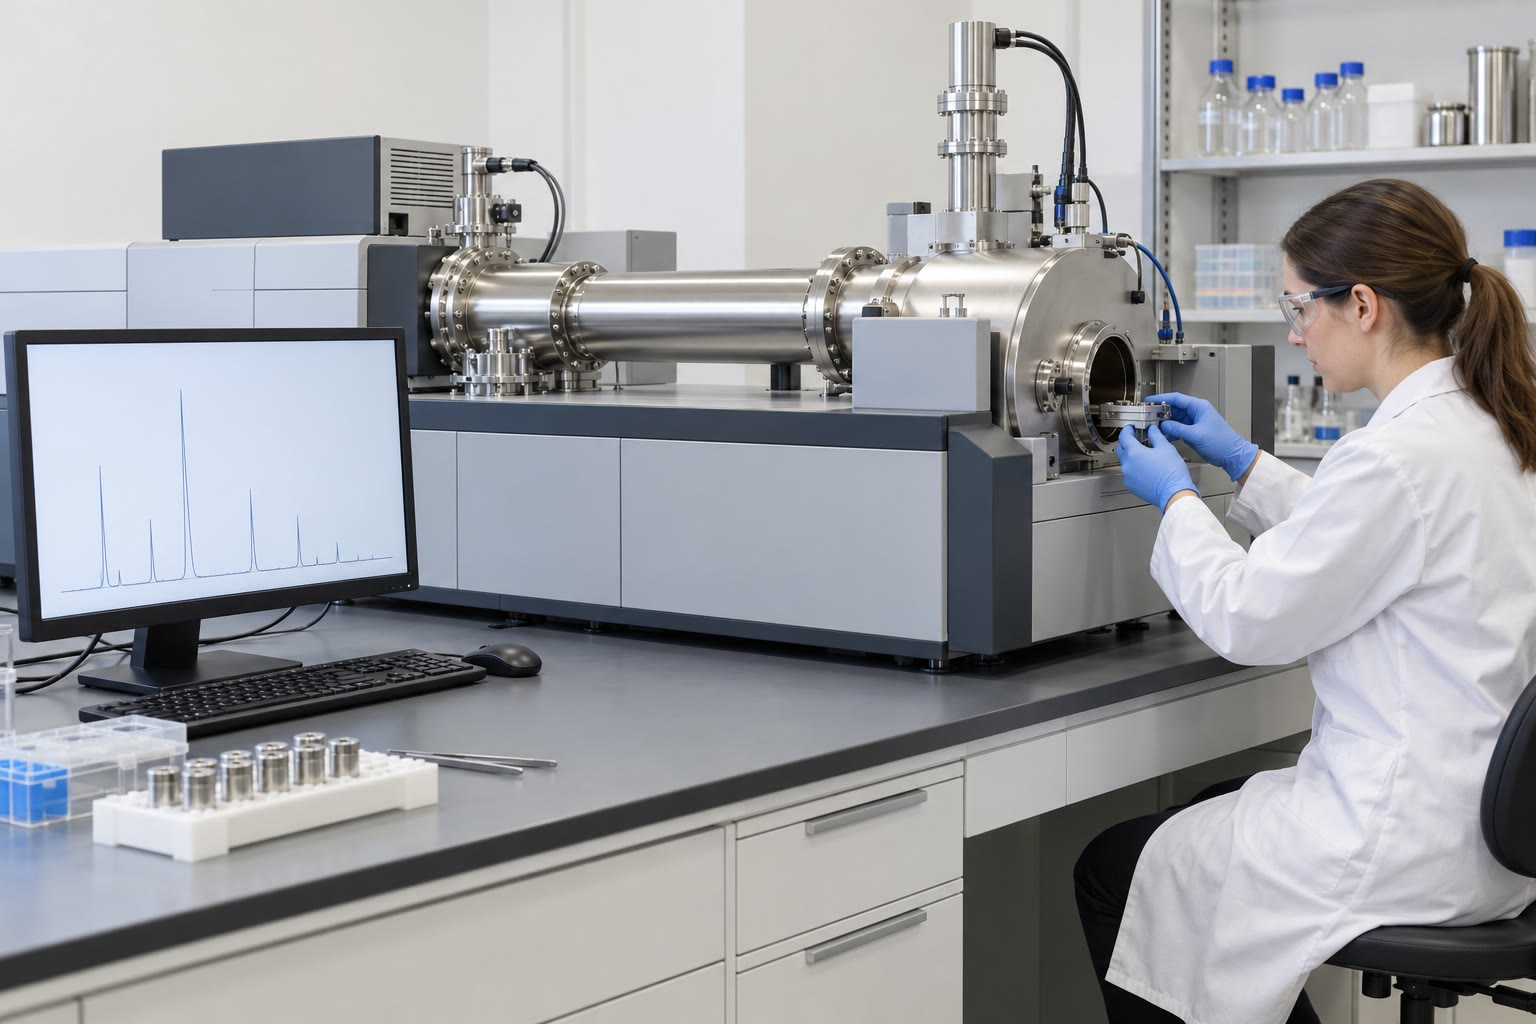
\includegraphics[width=0.66\linewidth]{images/book2/ai/g12-mass-spectrometer-lab.jpg}

{\small Un spectromètre de masse dans un laboratoire~: on charge un
échantillon du côté de la source. Illustration générée par IA.}
\end{omfigure}

Le rapport initial renseigne aussi sur l'origine du magma. Quand le manteau
fond, le rubidium passe de préférence dans le liquide~; au fil des âges, il
s'est donc concentré dans la \omterm{def:g12:continental-crust:continental-crust}{croûte continentale}, qui a ainsi produit
davantage de strontium~87~: les roches crustales ont un rapport
$^{87}\mathrm{Sr}/^{86}\mathrm{Sr}$
plus élevé que les roches du manteau. Un magma issu de la fusion de la
croûte hérite de ce rapport élevé.
% ledger: tulane:radiometric

\section{L'âge de la Terre}

Aucune roche terrestre ne remonte aux débuts de la Terre~: la plus vieille
roche connue, le gneiss d'Acasta, a 4.03~milliards d'années, et les plus
vieux zircons 4.4~milliards. La surface a depuis été fondue, érodée et
recyclée. La datation de la Terre elle-même vient des météorites,
fragments des petits corps qui se sont formés avec les planètes et dont
certains sont restés des \omterm{def:g12:age-of-the-earth:closed-system}{systèmes clos} depuis.
% ledger: bowring99:acasta, wilde01:zircon, usgs:age-earth (Book 1 row)

\begin{definition}[Âge de la Terre]\label{def:g12:age-of-the-earth:age}
L'\emph{âge de la Terre}\index{age de la Terre@âge de la Terre} est le
temps écoulé depuis que la Terre s'est formée par accrétion de corps plus
petits, à la naissance du système solaire. Mesuré sur les météorites par
datation radiométrique, il vaut \num{4.54}~milliards d'années, à un pour
cent près.
\end{definition}
% ledger: usgs:age-earth (Book 1 row)

En 1956, Clair Patterson mesura les isotopes du plomb de trois météorites
pierreuses et de deux météorites de fer. Deux isotopes du plomb sont
produits par la désintégration de l'uranium, le plomb~206 par
l'uranium~238 et le plomb~207 par l'uranium~235, tandis que le plomb~204
n'est produit par aucune désintégration. Comme pour le strontium, les
points de météorites formées en même temps sont alignés quand on porte
$^{207}\mathrm{Pb}/^{204}\mathrm{Pb}$ en fonction de
$^{206}\mathrm{Pb}/^{204}\mathrm{Pb}$. La météorite de fer de Canyon
Diablo, en Arizona, ne contient presque pas d'uranium~: son plomb n'a pas
changé depuis sa formation, et marque l'extrémité inférieure de la droite,
le plomb avec lequel le système solaire a commencé.
% ledger: patterson56:table, patterson56:constants, usgs:age-earth (Book 1 row: Canyon Diablo troilite)

\begin{omfigure}
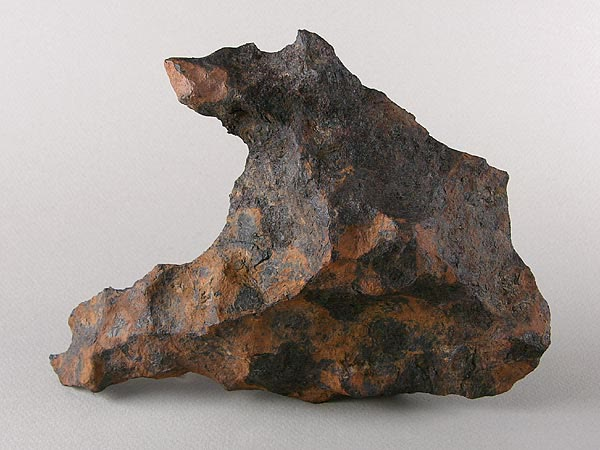
\includegraphics[height=4.2cm]{images/book2/g12-canyon-diablo-meteorite.jpg}

{\small Un fragment de la météorite de fer de Canyon Diablo,
\qty{2641}{g}. Photographie Geoffrey Notkin, CC~BY-SA~2.5 (Wikimedia
Commons).}
\end{omfigure}
% ledger: photo:g12-canyon-diablo

Pour le plomb, la pente $m$ dépend de l'âge par l'intermédiaire des deux
isotopes de l'uranium~; on admet ici la relation. Avec les constantes
qu'utilisait Patterson,
\[
  m = \frac{1}{137.8}\,\frac{e^{\lambda_{235}t}-1}{e^{\lambda_{238}t}-1},
  \qquad \lambda_{235} = \num{9.72e-10},\ \lambda_{238} = \num{1.537e-10}
  \text{ par an},
\]
ce qui donne~:
\begin{center}
\small
\begin{tabular}{|l|c|c|c|c|c|c|}
\hline
âge (milliards d'années) & 4.40 & 4.45 & 4.50 & 4.55 & 4.60 & 4.65 \\
pente $m$ & 0.533 & 0.551 & 0.570 & 0.590 & 0.610 & 0.632 \\
\hline
\end{tabular}
\end{center}
% ledger: patterson56:constants
% values: pb_slope at 4.40-4.65 Ga (isochrons.py pb_slope)

\begin{omfigure}
\begin{tikzpicture}
\begin{axis}[omrecord, width=0.72\linewidth, height=6cm, xmin=0, xmax=56, ymin=0, ymax=40,
  xlabel={$^{206}\mathrm{Pb}/^{204}\mathrm{Pb}$}, ylabel={$^{207}\mathrm{Pb}/^{204}\mathrm{Pb}$}]
% computed in figdata/grade-12/isochrons.py; ledger: patterson56:table
\addplot[omDef, line width=0.9pt] table[x=x, y=y] {figdata/out/grade-12-isochrons-pbln.dat};
\addplot[omThm, only marks, mark=*, mark size=2pt] table[x=r206, y=r207, restrict expr to domain={\thisrow{idx}}{1:5}] {figdata/out/grade-12-isochrons-pbpb.dat};
\addplot[black, only marks, mark=o, mark size=2.6pt, line width=0.8pt] table[x=r206, y=r207, restrict expr to domain={\thisrow{idx}}{6:6}] {figdata/out/grade-12-isochrons-pbpb.dat};
\coordinate (nl) at (axis cs:50.28,34.86);
\coordinate (fc) at (axis cs:19.48,15.76);
\coordinate (cd) at (axis cs:9.5,10.36);
\coordinate (sed) at (axis cs:19.0,15.5);
\coordinate (sl) at (axis cs:30,25);
\end{axis}
\node[font=\scriptsize, anchor=north west] at ([xshift=2pt]nl) {Nuevo Laredo};
\node[font=\scriptsize, anchor=north west, align=left] at ([xshift=4pt, yshift=-2pt]fc) {Forest City, Modoc~;\\sédiment océanique (cercle)};
\node[font=\scriptsize, anchor=north west, align=left] at ([xshift=3pt, yshift=-3pt]cd) {Canyon Diablo, Henbury (fer)};
\node[font=\scriptsize, text=omDef, anchor=south east] at (sl) {pente 0.603~: environ 4.6~milliards d'années};
\end{tikzpicture}

{\small L'\omterm{def:g12:age-of-the-earth:isochron}{isochrone} du plomb de Patterson~: les cinq météorites sont
alignées, et le plomb d'un sédiment océanique actuel, qui représente la
Terre, l'est presque aussi. Source~: Patterson (1956), tableau~1.}
\end{omfigure}
% values: pb_slope 0.6026, pb_age_Ga 4.58, sediment_residual -0.39 (isochrons.py)

Une droite tracée par les cinq points a une pente d'environ 0.603, entre
les pentes du tableau pour 4.55 et 4.60~milliards d'années. Le résultat de
Patterson lui-même, compte tenu des erreurs de mesure et des incertitudes
sur les constantes de désintégration, fut de 4.55~milliards d'années, à
0.07 près. Il mesura ensuite le plomb d'un sédiment océanique actuel, qui
mélange le plomb d'une grande masse de croûte terrestre~: il se place sur
la même droite. Le plomb de la Terre a évolué comme celui des météorites,
pendant la même durée~: la Terre a le même âge qu'elles.
% ledger: patterson56:table

Depuis, des centaines de mesures l'ont confirmé. Les météorites donnent
des âges de 4.53 à 4.58~milliards d'années, et les plus anciens solides du
système solaire, de petites inclusions riches en calcium et en aluminium
trouvées dans certaines météorites, se sont formés il y a \num{4567.30}
millions d'années, à 0.16 près. La Terre s'est formée plus tard à partir
de ce matériau~: c'est pourquoi son âge, 4.54~milliards d'années, est un
peu inférieur au leur.
% ledger: usgs:age-earth (Book 1 row), connelly12:cai

\section{Exercices}

\begin{exercise}[$\star$]\label{exo:g12:age-of-the-earth:1}
Donner le mot~: (a) un minéral dans lequel aucun atome père ou fils n'est
entré ni dont aucun n'est sorti depuis que son horloge s'est mise en
marche~; (b) la droite sur laquelle se placent les minéraux d'un même âge
et d'une même source~; (c) le temps écoulé depuis que la Terre s'est
formée par accrétion.
\end{exercise}

\begin{exercise}[$\star$]\label{exo:g12:age-of-the-earth:2}
À l'aide du tableau du granite de Varden, ranger ses cinq échantillons
dans l'ordre de leur rapport rubidium~87 sur strontium~86, du plus faible au
plus élevé. Lequel se place le plus haut sur l'\omterm{def:g12:age-of-the-earth:isochron}{isochrone}, et pourquoi
a-t-il produit le plus de strontium~87~?
\end{exercise}

\begin{exercise}[$\star$]\label{exo:g12:age-of-the-earth:3}
Calculer la demi-vie du rubidium~87 à partir de sa constante de
désintégration, \num{1.3972e-11} par an. Combien de fois l'\omterm{def:g12:age-of-the-earth:age}{âge de la Terre}
représente-t-elle~?
\end{exercise}

\begin{exercise}[$\star$]\label{exo:g12:age-of-the-earth:4}
Calculer $e^{\lambda t} - 1$ pour le rubidium~87 avec $t = 310$ millions
d'années et $t = 480$ millions d'années.
\end{exercise}

\begin{exercise}[$\star$]\label{exo:g12:age-of-the-earth:5}
Ranger par ordre de date les estimations de Phillips, de Holmes (1927), de
Joly, de Kelvin (1862) et de Patterson. Combien de fois l'âge actuel de la
Terre est-il plus grand que la borne supérieure de l'estimation de Joly~?
\end{exercise}

\begin{exercise}[$\star\star$]\label{exo:g12:age-of-the-earth:6}
Un minéral du granite de Varden (310 millions d'années, rapport initial
0.7080) a $^{87}\mathrm{Rb}/^{86}\mathrm{Sr} = 10.0$. Quel est
aujourd'hui son rapport $^{87}\mathrm{Sr}/^{86}\mathrm{Sr}$~? Quel était-il
quand le granite s'est formé~?
\end{exercise}

\begin{exercise}[$\star\star$]\label{exo:g12:age-of-the-earth:7}
Quatre échantillons du schiste de Varden donnent $(x, y)$ = (0.90, 0.71806),
(2.60, 0.72950), (5.10, 0.74632) et (9.40, 0.77525), avec $x =
{}^{87}\mathrm{Rb}/^{86}\mathrm{Sr}$ et $y = {}^{87}\mathrm{Sr}/^{86}\mathrm{Sr}$.
(1) À partir du premier et du dernier échantillon, calculer la pente et
l'âge. (2) Vérifier que les deux échantillons du milieu sont sur la même
droite. (3) Le résultat est-il cohérent avec les 310 millions d'années du
granite et avec le principe de recoupement~?
\end{exercise}

\begin{exercise}[$\star\star$]\label{exo:g12:age-of-the-earth:8}
Pourquoi une roche dont tous les minéraux ont le même rapport du rubidium
au strontium ne donne-t-elle aucune \omterm{def:g12:age-of-the-earth:isochron}{isochrone}~? Pourquoi la biotite, dans
le granite de Varden, fixe-t-elle mieux la pente que les autres minéraux~?
\end{exercise}

\begin{exercise}[$\star\star$]\label{exo:g12:age-of-the-earth:9}
Longtemps après la formation du granite de Varden, un fluide chaud a fait
perdre à sa biotite une partie de son strontium~87. (1) Où son point se
déplace-t-il sur le diagramme \omterm{def:g12:age-of-the-earth:isochron}{isochrone}~? (2) Quel âge la biotite et le
plagioclase donneraient-ils alors à eux seuls~: trop vieux ou trop
jeune~? (3) Comment la méthode de l'\omterm{def:g12:age-of-the-earth:isochron}{isochrone} révèle-t-elle le problème~?
\end{exercise}

\begin{exercise}[$\star\star$]\label{exo:g12:age-of-the-earth:10}
(1) Combien de fois l'\omterm{def:g12:age-of-the-earth:age}{âge de la Terre} est-il plus long que les 96 millions
d'années de Kelvin~? (2) Joly supposait que les fleuves apportent du sel à
la mer à un rythme constant et qu'aucune partie n'en quitte la mer.
Laquelle de ces hypothèses, si elle est fausse, rend son âge trop court, et
pourquoi~?
\end{exercise}

\begin{exercise}[$\star\star$]\label{exo:g12:age-of-the-earth:11}
À l'aide des valeurs de Patterson pour Canyon Diablo (9.46, 10.34) et Nuevo
Laredo (50.28, 34.86), calculer la pente de la droite qui passe par les
deux météorites, et lire l'âge dans le tableau des pentes.
\end{exercise}

\begin{exercise}[$\star\star\star$]\label{exo:g12:age-of-the-earth:12}
Un basalte de la région de Varden, âgé lui aussi de 310 millions d'années,
a un rapport initial de 0.7035, contre 0.7080 pour le granite. (1) Quelle
roche provient plus probablement de la fusion du manteau, et laquelle de la
fusion de la croûte~? (2) Expliquer pourquoi, à l'aide de ce que l'on sait
du rubidium. (3) Les deux roches auraient-elles pu cristalliser à partir
d'un même magma~?
\end{exercise}

\begin{exercise}[$\star\star\star$]\label{exo:g12:age-of-the-earth:13}
(1) Quelle fraction du rubidium~87 présent à la formation de la Terre
reste-t-il aujourd'hui~? Et de l'uranium~238 (demi-vie 4.47~milliards
d'années)~? (2) Quelle serait la pente d'une \omterm{def:g12:age-of-the-earth:isochron}{isochrone} rubidium--strontium
pour une roche âgée d'un million d'années~? Pourquoi le couple
rubidium--strontium est-il une mauvaise horloge pour les roches jeunes~?
\end{exercise}

\begin{exercise}[$\star\star\star$]\label{exo:g12:age-of-the-earth:14}
La droite qui passe par les cinq météorites de Patterson a pour équation
$y = 4.438 + 0.6026\,x$. (1) Quel rapport $^{207}\mathrm{Pb}/^{204}\mathrm{Pb}$
prévoit-elle pour le sédiment océanique, à $x = 19.0$~? Patterson a
mesuré 15.5~: de quel pourcentage les deux valeurs diffèrent-elles~?
(2) Quel âge la pente 0.6026 donne-t-elle, d'après le tableau~? Comparer
aux $4.55 \pm 0.07$~milliards d'années de Patterson.
\end{exercise}

\begin{exercise}[$\star\star\star$]\label{exo:g12:age-of-the-earth:15}
Kelvin supposait que toute la chaleur que perd la Terre,
\qty{46.7}{TW} aujourd'hui, est de la chaleur emmagasinée. (1) La
radioactivité en remplace environ \qty{24.4}{TW}. De combien cela suffit-il
à allonger, à soi seul, le temps nécessaire pour perdre un stock de chaleur
donné~? (2) En partant de 96 millions d'années, cela suffit-il pour
atteindre l'âge véritable~? (3) Qu'est-ce que Kelvin a négligé, qui compte
davantage~?
\end{exercise}

\begin{problem}[{Problème du week-end --- dater le granite de Varden}]
\label{pb:g12:age-of-the-earth:1}
% exercise data from figdata/grade-12/isochrons.py; ledger: villa22:rb87, tulane:radiometric, ics:base.Carboniferous, ics:base.Permian
Le granite des collines de Varden, la région imaginaire de la série,
recoupe le schiste qui l'entoure. Un laboratoire a mesuré cinq de ses
échantillons (exemple ci-dessus)~: plagioclase (0.35, 0.70952), hornblende
(1.20, 0.71321), roche totale (3.10, 0.72146), feldspath potassique (6.40,
0.73578) et biotite (24.0, 0.81218), chacun sous la forme
$(^{87}\mathrm{Rb}/^{86}\mathrm{Sr},\ ^{87}\mathrm{Sr}/^{86}\mathrm{Sr})$. La
constante de désintégration du rubidium~87 vaut \num{1.3972e-11} par an.

\medskip
\noindent\textbf{Partie I --- Les échantillons.}
\begin{enumerate}
  \item Quel échantillon est le plus riche en rubidium par rapport au
        strontium~?
  \item Pourquoi tous les minéraux ont-ils commencé avec le même rapport
        $^{87}\mathrm{Sr}/^{86}\mathrm{Sr}$~?
  \item Pourquoi rapporte-t-on les quantités au strontium~86~?
  \item Lequel des trois isotopes a augmenté depuis la formation du
        granite, et pourquoi~?
  \item À quoi ressemblaient les cinq points sur le diagramme quand le
        granite venait de se former~?
\end{enumerate}

\medskip
\noindent\textbf{Partie II --- La droite isochrone.}
\begin{enumerate}[resume]
  \item Calculer la pente par le plagioclase et la biotite.
  \item Calculer la pente par le plagioclase et la roche totale.
  \item Comparer les deux pentes. Laquelle est la plus fiable, et pourquoi~?
  \item Trouver où la droite de la question 6 coupe l'axe vertical.
  \item Vérifier que le feldspath potassique est sur cette droite.
\end{enumerate}

\medskip
\noindent\textbf{Partie III --- La pente et l'âge.}
\begin{enumerate}[resume]
  \item Écrire la relation entre la pente et $e^{\lambda t}$.
  \item Calculer $\lambda t$.
  \item Calculer l'âge $t$.
  \item Le schiste a été daté de 480 millions d'années. L'ordre des deux
        âges est-il celui qu'exigent les relations de terrain~?
  \item Le Carbonifère s'étend de 358.9 à 298.9 millions d'années avant
        l'actuel. Au cours de quelle période le granite s'est-il formé~?
\end{enumerate}

\medskip
\noindent\textbf{Partie IV --- Le rapport initial et la source.}
\begin{enumerate}[resume]
  \item Que représente l'ordonnée à l'origine, 0.7080~?
  \item Un basalte de la région s'est formé avec un rapport de 0.7035.
        Quelle roche a le rapport initial le plus élevé~?
  \item Pourquoi les roches crustales ont-elles des rapports plus élevés
        que le manteau~?
  \item Que suggère le rapport initial du granite sur la roche qui a fondu
        pour le produire~?
  \item Résumer~: quel est l'âge du granite de Varden~?
\end{enumerate}
\end{problem}
